%
% File main.tex
%
% NLP course project-proposal template, Warsaw University of Technology.
% Prepared by Anna Wróblewska, adapted from the ACL 2015 conference
% formatting template (acl2015.sty), originally by the ACL 2015
% organizers and earlier ACL/EACL format authors (see acl2015.pdf
% for the full credits chain).

\documentclass[11pt]{article}
\usepackage{acl2015}
\usepackage{times}
\usepackage{url}
\usepackage{latexsym}
\usepackage{xcolor}

%\setlength\titlebox{5cm}

% You can expand the title box if you need extra space
% to show all the authors. Please do not make the title box
% smaller than 5cm (the original size); we will check this
% in the camera-ready version and ask you to change it back.
\usepackage{float}
\usepackage{tikz}
\usetikzlibrary{arrows.meta,positioning}

\title{Is LLM self-consistency a usable signal for routing annotation work?\\Project Proposal for NLP Course, Winter 2026/27}
% https://www.overleaf.com/project/63440c16442dba647b52a1ae
\author{Tymoteusz Urban \\
  Album number \\
  {\tt email@pw.edu.pl} \\\And
  Sebastian Trojan \\
  320664 \\
  {\tt 01171271@pw.edu.pl} \\ \And
  Mateusz Nizwantowski \\
  313839 \\
  {\tt 01161932@pw.edu.pl} \\ \AND
  supervisor: Soveatin Kuntur\\
  Warsaw University of Technology \\
  {\tt soveatin.kuntur.dokt@pw.edu.pl}}
\date{}

\begin{document}
\maketitle

\begin{abstract}
  Write about the proposed work touching the research gap you are addressing, novelty, and on the proposed deliverable aimed from this project.
  (Short description up to 250 words.)
\end{abstract}

\section{Introduction}
\begin{enumerate}
\item \textbf{Scientific goal of the project.}
This study asks whether self-consistency across LLM reruns predicts correctness of multilabel annotations of Polish persuasion and manipulation techniques and supports cost-effective human--model routing. H1: higher self-consistency distinguishes correct from incorrect predictions better than chance across models, datasets and prompting strategies. H2: at comparable annotation quality, consistency-based routing achieves greater automatic coverage than alternative confidence-based approaches, including cheaper single-run methods. We also evaluate risk--coverage trade-offs, human annotation effort saved and additional inference costs. Negative results are considered valid research outcomes.

\item \textbf{Significance of the project.}
Annotation is costly, but LLMs can be consistently wrong. Repeated inference also adds compute cost, so improved routing must be compared with cheaper confidence signals. We evaluate self-consistency for multilabel Polish text classification and its practical cost--quality trade-off. Model comparisons are descriptive, not causal evidence about size or language specialisation.

\item \textbf{Concept and work plan.}
Figure~\ref{fig:pipeline} summarises the workflow.

\begin{figure}[H]
\centering
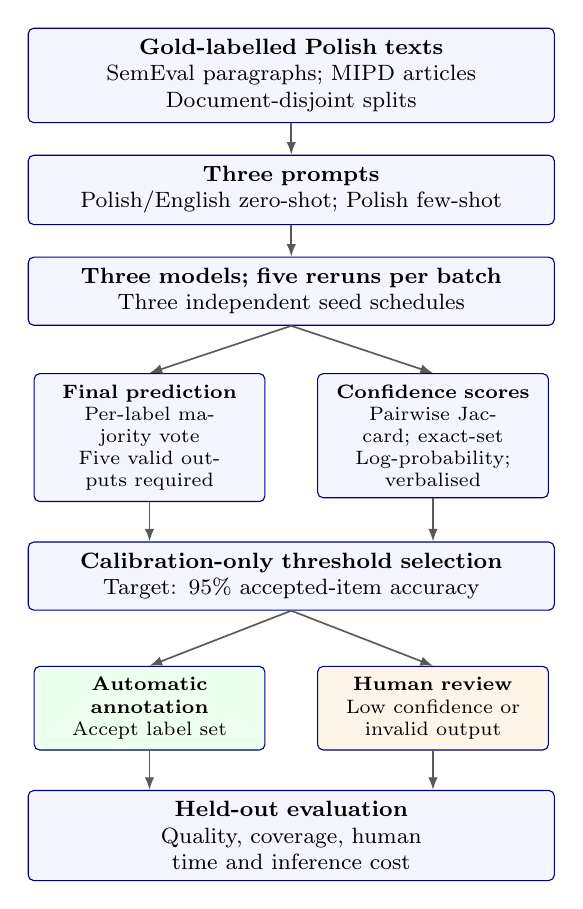
\begin{tikzpicture}[
  node distance=4mm,
  stage/.style={draw=blue!50!black,fill=blue!4,rounded corners=2pt,
    align=center,font=\footnotesize,text width=6.4cm,inner sep=4pt},
  branch/.style={stage,text width=2.65cm,font=\scriptsize},
  analysis/.style={branch,minimum height=1.55cm},
  flow/.style={-{Latex[length=1.6mm]},semithick,draw=black!65}]
\node[stage] (data) {\textbf{Gold-labelled Polish texts}\\SemEval paragraphs; MIPD articles\\Document-disjoint splits};
\node[stage,below=of data] (prompts) {\textbf{Three prompts}\\Polish/English zero-shot; Polish few-shot};
\node[stage,below=of prompts] (runs) {\textbf{Three models; five reruns per batch}\\Three independent seed schedules};
\node[analysis,below=6mm of runs.south,xshift=-1.8cm] (prediction)
  {\textbf{Final prediction}\\Per-label majority vote\\Five valid outputs required};
\node[analysis,below=6mm of runs.south,xshift=1.8cm] (signals)
  {\textbf{Confidence scores}\\Pairwise Jaccard; exact-set\\Log-probability; verbalised};
\node[stage,below=5mm of prediction.south,xshift=1.8cm] (routing)
  {\textbf{Calibration-only threshold selection}\\Target: 95\% accepted-item accuracy};
\node[branch,fill=green!7,below=7mm of routing.south,xshift=-1.8cm]
  (automatic) {\textbf{Automatic annotation}\\Accept label set};
\node[branch,fill=orange!9,below=7mm of routing.south,xshift=1.8cm]
  (human) {\textbf{Human review}\\Low confidence or\\invalid output};
\node[stage,below=5mm of automatic.south,xshift=1.8cm] (quality)
  {\textbf{Held-out evaluation}\\Quality, coverage, human time and inference cost};
\draw[flow] (data) -- (prompts);
\draw[flow] (prompts) -- (runs);
\draw[flow] (runs.south) -- (prediction.north);
\draw[flow] (runs.south) -- (signals.north);
\draw[flow] (prediction.south) -- ([xshift=-1.8cm]routing.north);
\draw[flow] (signals.south) -- ([xshift=1.8cm]routing.north);
\draw[flow] (routing.south) -- (automatic.north);
\draw[flow] (routing.south) -- (human.north);
\draw[flow] (automatic.south) -- ([xshift=-1.8cm]quality.north);
\draw[flow] (human.south) -- ([xshift=1.8cm]quality.north);
\end{tikzpicture}
\caption{Planned annotation-routing pipeline. Thresholds are calibrated without test labels; human correction is simulated with gold labels.}
\label{fig:pipeline}
\end{figure}

\textit{Three deliverables.}
(i) Consistency--correctness analyses per model, dataset and supported label, with uncertainty estimates and confidence baselines.
(ii) Risk--coverage and cost--quality curves, including comparison with single-run routing and a selected operating point (if feasible).
(iii) Reproducible prompts, code, settings and outputs; sensitive outputs remain private.

\textit{Preliminary status.}
Datasets and label definitions are available; model experiments have not yet been run.

\textit{Timeline and ownership.}
Table~\ref{tab:work-plan} presents weekly tasks, milestones and individual responsibilities.

\begin{table}[H]
\centering
\footnotesize
\begin{tabular}{@{}p{1.15cm}@{\hspace{5pt}}p{5.15cm}@{}}
\hline
Date & Planned output and owner\\
\hline
\textbf{04 Nov} &
\textbf{Phase 1:} Methodology and pipeline (S); SOTA (T); datasets and data statement (M).\\
11 Nov &
Docker/Conda/vLLM, GPU setup and data splits (M); inference pipeline and parsing (S); prompt preparation (T).\\
\textbf{18 Nov} &
\textbf{Mid-term:} Three-model pilot with five reruns (S,M); SOTA presentation and video (T); start main runs (M).\\
25 Nov &
Continue main inference (M); consistency metrics and confidence baselines (S); EDA and annotation-time sample (T).\\
\textbf{02 Dec} &
\textbf{Phase 2:} Main inference and reproducible MR/README (M); preliminary evaluation (S); report and rebuttals (T).\\
09 Dec &
Validate outputs and recover failures (M); AUC and confidence comparisons (S); preliminary error analysis (T).\\
16 Dec &
Routing, calibration and bootstrap (S); GPU performance measurements (M); 20+ classified errors (T).\\
23 Dec &
Risk--coverage and cost analysis (S); results discussion (T); reproducibility tests (M).\\
30 Dec &
Complete report draft (T); final figures and results (S); code and README audit (M).\\
06 Jan &
Final results verification (S); report revision and presentation video (T); final merge request (M).\\
\textbf{13 Jan} &
\textbf{Phase 3:} Final report, presentation, code and MR (S,T,M).\\
\hline
\end{tabular}
\caption{Weekly plan for 2026/27. S = Sebastian Trojan; T = Tymoteusz Urban; M = Mateusz Nizwantowski. All dates are Wednesdays; January dates refer to 2027.}
\label{tab:work-plan}
\end{table}

\textit{Risks and responses.}
Pilot runtime will determine a feasible shared sample and GPU settings. Audit data/model licences, missing labels and document leakage. Report rare-label limitations; route invalid outputs to humans. Record uncertainty and examine at least 20 misclassified examples grouped by error type.

\item \textbf{Approach and research methodology.}
\textit{Data and models.}
Use SemEval-2023 Task~3 Polish paragraphs and MIPD articles with separate native label taxonomies. Verify whether absent MIPD indicators mean negative or missing labels. Audit duplicates and enforce document-disjoint training, calibration and held-out splits; use official splits where possible. Models: Bielik 11B v3 Instruct (SpeakLeash), PLLuM 12B Chat 2412 (CYFRAGOVPL) and Gemma 4 E2B IT (Google).


\textit{Prompt strategies.}
Use Polish zero-shot, English zero-shot and Polish few-shot prompts with equivalent instructions, label IDs and output schemas. Few-shot examples come only from training data; comparisons isolate instruction language or demonstrations, not a full factorial design.

\textit{Repeated inference and failures.}
Generate five outputs per model, item and prompt using fixed stochastic settings and logged seeds. Replicate the main comparison using three independent five-output batches on a common pilot-sized sample, reporting the spread. Log raw and parsed outputs, versions and settings. Refer items with any invalid output to a human; report failures separately from classification accuracy and retain all items in coverage denominators.

\textit{Prediction and self-consistency.}
For five valid outputs, predict each label by majority vote. Measure exact-set agreement (modal-set frequency), mean pairwise Jaccard similarity over ten pairs (primary score), and per-label agreement. Confidence scores never use gold labels.

\textit{Confidence baselines.}
On the same voted predictions, compare self-consistency with length-normalised token log-probability of the canonical voted label set, scored by teacher forcing under the original prompt; verbalised confidence elicited on a fixed $[0,1]$ scale; and random routing. Log additional scoring/query costs. Report unavailable log-probability baselines explicitly.

\textit{Metrics and uncertainty.}
Report micro/macro-F1 and exact-set accuracy on valid predictions, plus failure rates. Evaluate ROC AUC for predicting exact-set correctness, supplemented by error-detection PR AUC. Analyse per-label correctness only with adequate support. Use paired document-level bootstrap 95\% confidence intervals and report spread across independent seed schedules.

\textit{Routing evaluation.}
Calibrate thresholds without test data, maximising coverage subject to 95\% accepted-item exact-set accuracy and a predeclared minimum accepted count; also examine 80\% and 90\% targets. Evaluate risk--coverage curves, accepted-only quality and final quality under ideal gold-based human correction on held-out data. Report infeasible targets instead of assuming coverage.

\textit{Cost--benefit analysis.}
Compare confidence signals on matched five-run predictions and complete policies against cheaper single-run baselines. Report coverage, quality, inference time and estimated human hours based on a timed sample from each dataset. Estimate net monetary cost using explicit labour and compute rates, including reruns and confidence queries; do not assume savings.

\textit{Tools.}
Use Python and vLLM on local NVIDIA GPUs, with a Dockerfile and Conda environment specification. Log versions, model settings, seeds, GPU memory, runtime and execution commands. No model fine-tuning is planned.

\item well-justified project literature (full bibliographic data);
\item \textbf{Data statement.} Source, licence, personal data and safeguards (up to six lines).

\item \textbf{Contribution table.}
Table~\ref{tab:contributions} records Phase 1 work.
\begin{table}[H]
\centering
\footnotesize
\begin{tabular}{@{}p{1.9cm}@{\hspace{3pt}}p{3.7cm}@{\hspace{3pt}}p{0.5cm}@{}}
\hline
Member & Phase 1 contribution & h\\
\hline
\shortstack[l]{Tymoteusz\\Urban} & State-of-the-art literature review. & 8\\
\shortstack[l]{Sebastian\\Trojan} & Scientific goal, concept, methodology, plan, contribution table and LLM-use declaration. & 5\\
\shortstack[l]{Mateusz\\Nizwantowski} & Datasets and status; data statement. & 8\\
\hline
Total & & 17\\
\hline
\end{tabular}
\caption{Phase 1 division of work.}
\label{tab:contributions}
\end{table}

\item \textbf{Declaration of LLM use.}
OpenAI Codex supported drafting, language editing and \LaTeX{} formatting. The authors are responsible for the final content.
\end{enumerate}

% include your bib file like this:
%\bibliographystyle{acl}
%\bibliography{acl2015}

\end{document}